% ----- Basics Config -----
\documentclass{book}
\usepackage[utf8]{inputenc}
\usepackage{verbatim}
\usepackage{xcolor}

% ----- Math -----
\usepackage{minted}
\usepackage{amsmath}
\usepackage{mathtools}
\usepackage{amsfonts}
\usepackage{polynom}

% ----- Plots & Graphs -----
\usepackage{tikz}
\usetikzlibrary{calc, matrix, shapes.geometric, arrows}
\tikzstyle{startstop} = [rectangle, rounded corners, minimum width=3cm, minimum height=1cm,text centered, draw=black, fill=red!30]
\tikzexternalize
\usepackage{pgfplots}
\pgfplotsset{width=10cm,compat=1.9}
\usepgfplotslibrary{external}
\usepackage{graphicx}

% ----- Tables -----
\usepackage{longtable}
\usepackage{multirow}

% ----- Theorems -----
\newtheorem{defn}{Definição}
\numberwithin{defn}{chapter} 
\newtheorem{exe}{Exemplo}
\numberwithin{exe}{chapter} 
\newtheorem{ex}{Exercício}
\numberwithin{ex}{chapter} 
\newtheorem{obs}{Observação}
\numberwithin{obs}{chapter} 
\newtheorem{fato}{Fato}
\newtheorem{teo}{Teorema}
\numberwithin{fato}{chapter} 
\newtheorem{resp}{Resposta}
\numberwithin{resp}{chapter}
\newtheorem{prop}{Proposição}
\newtheorem{dem}{Demonstração}
\newtheorem{cor}{Corolário}
\newtheorem{exp1}{Exercício}
\newtheorem{exs1}{Exercício}

% ----- Title/author/date -----
\title{Cálculo - Notas de Aula}
\author{Prof. Me. Alexandre Garcia de Oliveira}
\date{Novembro 2022}

% ----- Document -----
\begin{document}
\maketitle

% ----- Content -----
% -------------------- Pré-Cálculo ------------------------
% \chapter{Pré-Cálculo}

% -------------------- Limites ------------------------
\chapter{Limites}

Neste capítulo será introduzido intuitivamente a noção de "limites". Mais adiante será de grande relevância para a continuidade do cálculo.

\section{Noção Intuitiva de Limite}
Para começar, um limite mensura o comportamento de uma função $f \text{ }\mathbb R \rightarrow \mathbb R$ em uma vizinhança de um ponto $a \in\mathbb R$.
\begin{center} $\lim\limits_{x\to a}f(x)$ \end{center}

\begin{exe} Considere $f(x) = x+1$ $\rightarrow \lim\limits_{x\to 1} x+1=2$. O gráfico dessa função ficaria representado da seguinte forma:
\begin{center}
\begin{tikzpicture}
\begin{axis}[xmin=-5, xmax=5, ymin=-5, ymax=5, axis x line=middle, axis y line=middle]
\addplot[domain=-5:5]{2*x + 1*x};
\end{axis}
\end{tikzpicture}
\end{center} 

\begin{longtable}[c]{| c | c |}
\caption{Quadro de limites.\label{long}}\\

\hline
\multicolumn{2}{| c |}{$\lim\limits_{x\to 2^{-}}f(x)=1$}\\
\hline
x & f(x)\\
\hline
\endfirsthead

\hline
\multicolumn{2}{|c|}{Continuation of Table \ref{long}}\\
\hline
Something & something else\\
\hline
\endhead

\hline
\endfoot

\hline
\multicolumn{2}{| c |}{}\\
\hline\hline
\endlastfoot

1.01 & 2.01\\
1.001 & 2.001\\
1.0001 & 2.0001\\
1.00001 & 2.00001\\
\end{longtable}

\begin{longtable}[c]{| c | c |}
\caption{Quadro de limites.\label{long}}\\

\hline
\multicolumn{2}{| c |}{$\lim\limits_{x\to 2^{+}}f(x)=2$}\\
\hline
x & f(x)\\
\hline
\endfirsthead

\hline
\multicolumn{2}{|c|}{Continuation of Table \ref{long}}\\
\hline
Something & something else\\
\hline
\endhead

\hline
\endfoot

\hline
\multicolumn{2}{| c |}{}\\
\hline\hline
\endlastfoot

0.9 & 1.9\\
0.99 & 1.99\\
0.999 & 1.999\\
0.9999 & 1.9999\\
\end{longtable}
\end{exe}

Através desse exemplo foi possível verificar que os limites escrevem-se de um ponto $a\in\mathbb{R}$, da forma:
\begin{center}
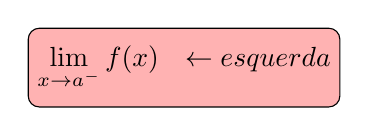
\begin{tikzpicture}[node distance=2cm]
\node (start) [startstop] {$\lim\limits_{x\to a^{-}}f(x)$ $\text{ } \leftarrow esquerda$};
\end{tikzpicture}
\end{center}

\begin{center}
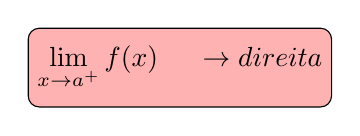
\begin{tikzpicture}[node distance=2cm]
\node (start) [startstop] {$\lim\limits_{x\to a^{+}}f(x)$ $\text{ } \text{ } \text{ } \rightarrow direita$};
\end{tikzpicture}
\end{center}

% Incluir gráfico 2

% Incluir gráfico 3

\textbf{NOTA:} O "limite" faz enconstar no zero enquanto a "derivada" pega os cantos.

\begin{defn}
    Uma função $f: \text{ }\mathbb R \rightarrow \mathbb R$ é dita contínua em um ponto $a \in\mathbb R$ se: 
\[\lim\limits_{x\to a^{+}}f(x) = \lim\limits_{x\to a^{-}}f(x)\]

\item Ou seja, existe 
\[\lim\limits_{x\to a}f(x)\] 
\end{defn}

\textbf{OBSERVAÇÃO:} Só é contínua se a mesma for contínua em $\textcolor{red}{todos}$ os pontos de seu domínio (injetora, sobrejetora?).

Se a função for contínua em $a\in\mathbb{R}$ então:
\[\lim\limits_{x\to a}f(x)=f(a)\]

Lembre-se de questionar qual é o argumento. Além disso, não é possível realizar uma função "sobrejetora".

\[\]
\textbf{NOTA:} $+\infty\notin\mathbb{R}$ e $-\infty\notin\mathbb{R}$, ou seja, infinito não é real. 

O mundo físico é "finito".
\[\]

\textbf{DICA} Você pode consultar a lista dos \textcolor{red}{tipos de funções contínuas} no livro de Cálculo, volume 1, do Gerge B. Thomas na página 124.


\begin{exe} Vejamos mais alguns casos:

a) $\lim\limits_{x\to 7} x^{4-1} = 1^4 -1 = 0$

b) $\lim\limits_{x\to 2}7=7$

c) $\lim\limits_{x\to 0} x^2-4x+1 = 0^2-4+1=1$

d) $\lim\limits_{x\to 0} senx=sen 0=0$

e) $\lim\limits_{x\to 0} cosx=cos 0=1$

f) $\lim\limits_{x\to 0}\frac{x-1}{x^2}=-\infty$

g) $\lim\limits_{x\to 0^{-}}\frac{x-1}{x^2}=-\infty$

h) $\lim\limits_{x\to 0^{+}}\frac{x-1}{x^2}=-\infty$
\[\]
Vejamos o próximo item detalhadamente:

i) $\lim\limits_{x\to 0}\frac{x-1}{x^3}=-\infty$
\begin{longtable}[c]{| c | c |}
\caption{Quadro de limites.\label{long}}\\

\hline
\multicolumn{2}{| c |}{$\lim\limits_{x\to 2^{+}}f(x)=2$}\\
\hline
x & f(x)\\
\hline
\endfirsthead

\hline
\multicolumn{2}{|c|}{Continuation of Table \ref{long}}\\
\hline
Something & something else\\
\hline
\endhead

\hline
\endfoot

\hline
\multicolumn{2}{| c |}{}\\
\hline\hline
\endlastfoot

0.1 & -500\\
0.01 & -98999\\
0.001 & $-9*10^8$\\
\end{longtable}

\[\lim\limits_{x\to 0^{+}}\frac{x-1}{x^3}=-\infty\]

\begin{longtable}[c]{| c | c |}
\caption{Quadro de limites.\label{long}}\\

\hline
\multicolumn{2}{| c |}{$\lim\limits_{x\to 2^{+}}f(x)=2$}\\
\hline
x & f(x)\\
\hline
\endfirsthead

\hline
\multicolumn{2}{|c|}{Continuation of Table \ref{long}}\\
\hline
Something & something else\\
\hline
\endhead

\hline
\endfoot

\hline
\multicolumn{2}{| c |}{}\\
\hline\hline
\endlastfoot

0.1 & 1100\\
0.01 & 100000\\
\end{longtable}

\[\lim\limits_{x\to 0^{-}}\frac{x-1}{x^3}=+\infty\]

\textbf{NOTA:} Quando os dois lados são "menos infinito", isso quer dizer que \textcolor{red}{não existe}.

\item\textbf{Propriedades do limite:}
\item 1. $\lim\limits_{x\to a}f(x)$, quando existe é único.
\item 2. Se k é constante, $\lim\limits_{x\to a}k=k$.
\item 3. $\lim\limits_{x\to a}[f(x)\pm g(x)] = \lim\limits_{x\to a}f(x)\pm \lim\limits_{x\to a}g(x)$.
\item 4. $\lim\limits_{x\to a}[k\cdot f(x)] = k\cdot \lim\limits_{x\to a}f(x)$.
\item 5. $\lim\limits_{x\to a}[f(x)\cdot g(x)] = \lim\limits_{x\to a}f(x)\cdot \lim\limits_{x\to a}g(x)$.
\item 6. $\lim\limits_{x\to a}[f(x)]^n = \lim\limits_{x\to a}[f(x)]^n$ $\rightarrow Lembre-se \text{ }da \text{ } propriedade\text{ } \sqrt[n]{f(x)}=[f(x)]^{\frac{1}{n}}$.
\item 7. $\lim\limits_{x\to a}\left[\frac{f(x)}{g(x)}\right] = \frac{\lim\limits_{x\to a}f(x)}{\lim\limits_{x\to a}g(x)}$, sendo $g(x)\text{ }\neq 0$.
\item 8. Teorema do confronto, sendo x e a $\in Df$ e $f(x)\le g(x)\le h(x)$, quando $\lim\limits_{x\to a}f(x) = \lim\limits_{x\to a}h(x) = b$, então $\lim\limits_{x\to a}g(x) = b$.
\end{exe}

\begin{exe}
    $\lim\limits_{x\to 1}(x^4-1) = (1)^4-1=0$ $\rightarrow$ Polinômio, função contínia. Basta calcular f(a).
\end{exe}

\begin{exe}
    $\lim\limits_{x\to 2}7 = 7$ $\rightarrow$ Limite de uma função.
\end{exe}

\begin{exe}
    $\lim\limits_{x\to 0}(x^2-4x+1) = (0)^2-4\cdot(0)+1=1$ $\rightarrow$ Polinômio.
\end{exe}

\begin{exe}
    $\lim\limits_{x\to 0}(sen x) = sen(0)=0$ $\rightarrow$ Função trigonométrica.
\end{exe}

\begin{exe}
    $\lim\limits_{x\to 0}(cos x) = cos(0)=1$ $\rightarrow$ Função trigonométrica.

\item\textbf{Observação:} Nem todas as funções trigonométricas são contínuas em seu domínio.
\end{exe}

Quando uma função não for uma das conhecidas, teremos de analisar os limites laterais da mesma.


% -------------------- Limites Indeterminados ------------------------

\section{Limites indeterminados} 
São limites da forma:

\[\lim\limits_{x\to a}\frac{f(x)}{g(x)}=\frac{0}{0}\]

Para resolver limites dessa forma, devemos manipular a expressão $\lim\limits_{x\to a}\frac{f(x)}{g(x)}$ até que a indeterminação $\frac{0}{0}$ suma.

As indeterminações podem ser levantadas por alguns processos algébricos, os quais não existe apenas uma maneira de calcular, pois cada caso deve ser analisado.

\begin{exe}
    %resolver um por divisão de polinômios
\end{exe}

% -------------------- Briot Ruffini ------------------------
\section{Briot-Ruffini}
\text{ }

Uma das técnicas de se resolver o limite indeterminado é por "Briot-Ruffini", a qual cosiste na aplicação de um algoritmo que auxilia na divisão dos polonômios.

Vejamos um exemplo:

\begin{exe} Considere o $\lim\limits_{x\to 3}\frac{x^4-x-78}{x^2-5x+6}$ e calcule por "Briot-Ruffini".

Primeiramente, note que temos um polinômio de 4° grau da forma $ax^4+bx^2+c=0$. Então, precisamos fatorar o g(x) de tal forma que possamos aplicar o algoritmo para resolver esse polinômio.

\item\textbf{DICA:} Sugiro que você revise as técnicas de "fatoração". 

\item\textbf{Primeiro passo:} Fatorando o g(x):
\[\lim\limits_{x\to 3}\frac{x^4-x-78}{x^2-5x+6} = \lim\limits_{x\to 3}\frac{x^4-x-78}{(x-2)(x-3)}\]

\item\textbf{Segundo passo:} Agora basta escolher um dos binômios para aplicar o método. Vamos escolher o $(x-3)$ e deixar o outro de lado.

\begin{center}
  \polyhornerscheme[x=3]{x^4-x-78}
\end{center}

\item\textbf{Terceiro passo:} Isso feito, é só analisar o algoritmo e substituir os valores encontrados no polinômio.

    \[\lim\limits_{x\to 3}\frac{x^3-3x^2+9x+26}{(x-2)} = \lim\limits_{x\to 3}\frac{3^3-3\cdot 3^2+9\cdot 3+26}{(3-2)} = 107\]

\[\]
\item\textbf{Resumo das indeterminações que poderemos encontrar}:
\item 1. $\infty \text{ } -\infty$.
\item 2 $0\cdot \infty$.
\item 3. $\frac{0}{0}$.
\item 4. $\frac{\infty}{\infty}$.
\item 5. $0^0 \text{ }\text{ }\infty^0$.
\item 6. $1^\infty$.
\end{exe}

% -------------------- Exercícios resolvidos ------------------------

\section{Exercícios}
\begin{ex}
    $\lim\limits_{x\to 7}\frac{x^3-14x^2+41+56}{x^2-9x+14}$.   
\end{ex}
\begin{ex}
    $\lim\limits_{x\to 1}\frac{x^5-3x^4-5x^3+15x^2+4x-12}{x^3-8x^2-11x+18}$.   
\end{ex}
\begin{ex}
    $\lim\limits_{x\to 2}\frac{x^4+x-18}{x^2-13x+22}$.   
\end{ex}

\section{Limites no Infinito} 
São limites na forma:

\begin{align*}
\lim\limits_{x\to + \infty}f(x) \\
\lim\limits_{x\to - \infty}f(x)  
\end{align*}

\begin{exe}
Calcule $\lim\limits_{x\to + \infty}f(x)$, onde $f(x)=\frac{1}{x^2}$

\begin{longtable}[c]{| c | c |}
\caption{Quadro de limites.\label{long}}\\

\hline
\multicolumn{2}{| c |}{$\lim\limits_{x\to 2^{+}}f(x)=2$}\\
\hline
x & f(x)\\
\hline
\endfirsthead

\hline
\multicolumn{2}{|c|}{Continuation of Table \ref{long}}\\
\hline
Something & something else\\
\hline
\endhead

\hline
\endfoot

\hline
\multicolumn{2}{| c |}{}\\
\hline\hline
\endlastfoot

1 & $\frac{1}{1^2}$=1\\
10 & $\frac{1}{10^2}$=0,01\\
100 & $\frac{1}{100^2}$=0,0001
\end{longtable}

Portanto, $\lim\limits_{x\to +\infty} \frac{1}{x^2}=0$. Isso nos diz que quanto maior o valor de X, menor será o valor de f(x). Quanto maior esse valor, mais próximo de será zero.
\end{exe}

\begin{exe}
Calcule o $\lim\limits_{x\to + \infty}\frac{1}{x}$.

\begin{longtable}[c]{| c | c |}
\caption{Quadro de limites.\label{long}}\\

\hline
\multicolumn{2}{| c |}{$\lim\limits_{x\to 2^{+}}f(x)=2$}\\
\hline
x & f(x)\\
\hline
\endfirsthead

\hline
\multicolumn{2}{|c|}{Continuation of Table \ref{long}}\\
\hline
Something & something else\\
\hline
\endhead

\hline
\endfoot

\hline
\multicolumn{2}{| c |}{}\\
\hline\hline
\endlastfoot

1 & $\frac{1}{1^2}$=1\\
10 & $\frac{1}{10^2}$=0,1\\
100 & $\frac{1}{100^2}$=0,001
\end{longtable}
\begin{longtable}[c]{| c | c |}
\caption{Quadro de limites.\label{long}}\\

\hline
\multicolumn{2}{| c |}{$\lim\limits_{x\to 2^{+}}f(x)=2$}\\
\hline
x & f(x)\\
\hline
\endfirsthead

\hline
\multicolumn{2}{|c|}{Continuation of Table \ref{long}}\\
\hline
Something & something else\\
\hline
\endhead

\hline
\endfoot

\hline
\multicolumn{2}{| c |}{}\\
\hline\hline
\endlastfoot

-1 & $\frac{1}{1^2}$=-1\\
-10 & $\frac{1}{10^2}$=-0,1\\
-100 & $\frac{1}{100^2}$=-0,001
\end{longtable}

Portanto, $\lim\limits_{x\to +\infty} \frac{1}{x}=0$ e $\lim\limits_{x\to -\infty} \frac{1}{x}=0$. de será zero.
\end{exe}

\begin{exe}
Calcule o $\lim\limits_{x\to + \infty}x$.

\[f(x)=+\infty\]

Portanto, $\lim\limits_{x\to +\infty}x=+\infty$ e $\lim\limits_{x\to -\infty}x=-\infty$. de será zero.
\end{exe}

\begin{ex}
    Para casa: usando a definição, deduza a derivada de $f(x)=ax^3+bx^2+cx+d$.
\end{ex}

% -------------------- Teorema de Bolzano ------------------------
\section{Teorema de Bolzano} 

Suponha uma função $f:\mathbb{R}\to\mathbb{R}$ contínua e sendo a e b $\in \mathbb{R}$, tal que:

$f(a)\cdot f(b)<0 \to$ existe um número ímpar de raízes reais no intervalo $]a,b[$. 
 
$f(a)\cdot f(b)>0 \to$ se existir raízes, será um número par de raízes reais o intervalo $]a,b[$. 

\begin{exe}
    Dada a função $f(x)=x-(lnx)^2$ no intervalo $]0.1,1[$ encontrar a raiz no intervalo se esta existir.

\item Passo 1: $x_1=\frac{1+0,1}{2}=0,55$ $\to f(0,55)=0,19 \to >0$, então existe uma raiz no intervalo [0.1,0.55]

\item Passo 2: $x_2=\frac{0,55+0,1}{2}=0,325$ $\to f(0,325)=0,325-[ln(0,325)]^2\approx -0,94 \to <0$
\item Precisão: $\left| \frac{0,325-0,55}{0,325} \right| \approx 0,69$ (o ideal seria algo próximo a $10^{-3})$

\item Passo 3: $x_3=\frac{0,325+0,55}{2}=0,4375$ $\to f(0,4375)=0,4375-[ln(0,4375)]^2\approx -0,246 \to <0$ então a raiz está em [0.4375,0.55]
\item Precisão: $\left| \frac{0,4375-0,55}{0,4375} \right| \approx 0,26$ (Muito alta)

\item Passo 4: $x_4=\frac{0,4375+0,55}{2}=0,49375$ $\to f(0,49375)=0,4375-[ln(0,49375)]^2\approx -0,004 \to <0$ então a raiz está em [0.49375,0.55]
\item Precisão: $\left| \frac{0,49375-0,55}{0,49375} \right| \approx 0,28$

\item Passo 5: $x_5=\frac{0,49375+0,55}{2}=0,521875$ $\to f(0,521875)=0,521875-[ln(0,521875)]^2\approx 0,099 \to <0$ então a raiz está em [0.49375,0.521875]
\item Precisão: $\left| \frac{0,49375-0,521875}{0,49375} \right| \approx 0,069$

\item O correto seria continuar, porém a resolução já está extensa. Portanto vamos aceitar a precisão do último x calculado que é: 0,521875.
\end{exe}

Para casa, um desafio: resolver o exercício abaixo.
\begin{ex}
    Procure uma aproximação da raiz da equação dada para o intervalo $[0.1,1]$ $x^3+lnx+\sqrt{x}=0$.
\end{ex}

% -------------------- Derivada ------------------------

\chapter{Derivadas} % 1V
A derivada mensura a taxa de variação infinitesimal de uma função em um determinado ponto. No caso de uma função de uma variável, essa variação é a razão entre a saída e a entrada.
\[\frac{df}{dx} = f'(x) = \lim_{h \to 0} \frac{f(x+h) - f(x)}{h}\]


\begin{exe}
    Considere uma função $y=f(x)$ com o gráfico.
    
\begin{center}\includegraphics[scale=0.7]{.jpg}\end{center}

Sendo h o incremento, temos $B=(x+h),f(x+h)$ e com o segmento $\widehat{AB}$ tem-se que a reta secante à curva da função f(x).

Podemos então calcular o coeficiente angular da reta secante $m_s$ através do triângulo ABC.
\[\]

\end{exe}

%------------VER UM LUGAR PRA ISSO AQUI--------------

\textbf{Função constante:} \(f(x) = K\), onde \(K \in \mathbb{R}\)
\[f'(x) = lim_{x \to 0} \frac{f(x+h) - f(x)}{h} = \lim_{h \to 0} \frac{K - K}{h} = \lim_{h \to 0} 0 = 0\]

\textbf{Função identidade:} \(f(x) = X\)

\[f(x) = x\] 
\[f(x + h) = x + h\]
\[f'(x) = \lim_{h \to 0} \frac{f(x + h) - f(x)}{h} = \lim_{h \to 0} \frac{x + h - x}{h} = \lim_{h \to 0} \frac{h}{h} = 1\]

\textbf{Função linear:} \(f(x) = ax + b\)

\[f(x+h) = a(x + h) + b = ax + ah + b\]
\[f'(x) = \lim_{h \to 0} \frac{f(x + h) - f(x)}{h} = \lim_{h \to 0} \frac{ax + ah + b - (ax + b)}{h}\]
\[= \lim_{h \to 0} \frac{ax + ah + b - (ax + b)}{h} = \lim_{h \to 0} \frac{ah}{h} = \lim_{h \to 0} a = a\]

\textbf{Parábolas:} \(f(x) = X^2\)

\[f(x+h) = (x+h)^2 = x^2 + 2xh + h^2\]
\[f'(x) = \lim_{h \to 0} \frac{f(x+h) - f(x)}{h} = \lim_{h \to 0} \frac{x^2 + 2xh + h^2 - x^2}{h}\]
\[= \lim_{h \to 0} \frac{2xh + h^2}{h} = \lim_{h \to 0} \frac{2xh}{h} + \frac{h^2}{h} = \lim_{h \to 0} 2x + h = 2x\]



%------------ATÉ AQUI--------------

\section{Derivabilidade} % 
\section{Continuidade} % 
\textbf{Definição:} Seja \( F: \mathbb{R} \rightarrow \mathbb{R} \), \( F \) é dito contínua em um ponto \( a \) pertencente a \( \mathbb{R} \) se:

\begin{itemize}
    \item[a-)] Existe \( \lim_{x \to a} f(x) \)
    \item[b-)] \( \lim_{x \to a} f(x) = f(a) \)
\end{itemize}

\begin{exe} A função \( f(x) = 3x + 2 \) é contínua em \( x = 3 \):

\[
\lim_{x \to 3} 3x + 2 = 3 \times 3 + 2 = 11 = f(3)
\]
\end{exe}

\begin{exe} A função \( f(x) = \frac{1}{x} \) não é contínua em \( x = 0 \) porque:

\[
\lim_{x \to 0^+} \frac{1}{x} = +\infty
\]

\[
\lim_{x \to 0^-} \frac{1}{x} = -\infty
\]
Portanto, o limite não existe.
\end{exe}

\noindent Seja \( F: \mathbb{R} \rightarrow \mathbb{R} \) é dita contínua se ela for contínua em todo ponto \( a \) pertencente a \( \mathbb{R} \).

\begin{exe} A função \( f(x) = \frac{1}{x} \) é contínua em \( \mathbb{R} - \{0\} \) e descontínua em \( x = 0 \):

\[
f(x) = 
\begin{cases}
    1 & \text{se } x \geq 0 \\
    -1 & \text{se } x < 0
\end{cases}
\]

\[
\lim_{x \to 0^+} f(x) = 1
\]

\[
\begin{array}{|c|c|}
\hline
x & f(x) \\
\hline
0.1 & 1 \\
0.01 & 1 \\
0.001 & 1 \\
\hline
\end{array}
\]

\[
\lim_{x \to 0^-} f(x) = 1
\]

\[
\begin{array}{|c|c|}
\hline
x & f(x) \\
\hline
-0.1 & -1 \\
-0.01 & -1 \\
-0.001 & -1 \\
\hline
\end{array}
\]

\noindent A função \( f \) é contínua em \(\mathbb{R} \{0\}\) e descontínua em   \(\mathbb \{0\}\).
\end{exe}

\begin{exe}Considere a função f(x) = 
\begin{cases}
    3, & \text{se } x \leq 5 \\
    4, & \text{se } 5 \leq x \leq 7 \\
    5, & \text{se } x \geq 7
\end{cases}

\begin{tikzpicture}[scale=0.8]
% Eixos
\draw[->] (-1,0) -- (9,0) node[right] {$x$};
\draw[->] (0,-1) -- (0,6) node[above] {$f(x)$};
% Função
\draw[blue, thick] (-1,3) -- (5,3);
\draw[blue, thick] (5,4) -- (7,4);
\draw[blue, thick] (7,5) -- (9,5);
% Pontos
\filldraw[blue] (5,3) circle (2pt) node[above] {$(5,3)$};
\filldraw[blue] (7,4) circle (2pt) node[above] {$(7,4)$};
\filldraw[blue] (5,4) circle (2pt);
\filldraw[blue] (7,5) circle (2pt) node[above] {$(7,5)$};
% Intervalos
\draw[dashed] (5,0) -- (5,3);
\draw[dashed] (7,0) -- (7,4);
% Rótulos
\node[below] at (5,0) {$5$};
\node[below] at (7,0) {$7$};
\end{tikzpicture}

\[\lim_{x \to 5^-} f(x) = 3\] 
\[\lim_{x \to 5^+} f(x) = 4\] 
Ou seja, \[ \not\exists \lim_{x \to 5} f(x)\]
Em contrapartida,
\[\lim_{x \to 7^+} f(x) = 5\] 
\[\lim_{x \to 7^+} f(x) = 4\] 
Ou seja, \[ \exists \lim_{x \to 7} f(x)\]


\noindent\textbf{Conclusão:} \( f \) é contínua em \(\mathbb{R} \{5, 7\}\) e descontínua em   \(\mathbb \{5, 7\}\).
\end{exe}
\section{Derivadas Parciais} % 2V - 3V 

\textbf{Definição:} Seja \(f: \mathbb{R}^2 \rightarrow \mathbb{R}\), as derivadas parciais são dadas por: 
\[f'(x) = \lim_{h \to 0} \frac{f(x+h) - f(x)}{h}\]
\[\frac{\partial f}{\partial x}(x, y) = \lim_{h \to 0} \frac{f(x+h, y) - f(x,y)}{h}\]
\[\frac{\partial f}{\partial y}(x, y) = \lim_{h \to 0} \frac{f(x, y+h) - f(x,y)}{h}\]

\begin{exe} \(f(x, y) =x^2 + y^2\)\\

Para X como variável e Y como constante:

\[\frac{\partial f}{\partial x}(x, y) = \lim_{h \to 0} \frac{f(x+h, y) - f(x, y)}{h} = \lim_{h \to 0} \frac{(x + h)^2 + y^2 - (x^2 + y^2)}{h}\]

\[= \lim_{h \to 0} \frac{x^2 + 2xh + h^2 + y^2 - x^2 - y^2}{h} = \lim_{h \to 0} \frac{2xh + h^2}{h} = \lim_{h \to 0} \frac{2xh}{h} + \frac{h^2}{h}\]

\[= \lim_{h \to 0} (2x + h) = 2x + 0 = 2x\]\\

Para Y como variável e X como constante:

\[\frac{\partial f}{\partial y}(x, y) = \lim_{h \to 0} \frac{f(x, y+h) - f(x, y)}{h} = \lim_{h \to 0} \frac{x^2 + (y + h)^2 - (x^2 + y^2)}{h}\]

\[= \lim_{h \to 0} \frac{x^2 + y^2 + 2yh + h^2 - x^2 - y^2}{h} = \lim_{h \to 0} \frac{2yh + h^2}{h} = \lim_{h \to 0} \frac{2yh}{h} + \frac{h^2}{h}
\]

\[= 2y + h = 2y + 0 = 2y\]

\end{exe}

\section{Derivada Parcial de um ponto} 
\textbf{Definição:} Pode-se calcular a derivada parcial em um ponto qualquer, por exemplo:
\[f(x, y) = xy\]
\[\frac{\partial f}{\partial x} = y\]
\[\frac{\partial f}{\partial x} = 7\]
Ou seja, a variação da função \(f\) em relação ao eixo no ponto (1,7) é 7.



\section{Exercícios}
\begin{ex}
Derive:
\item 1.1 $f(x)=\sqrt{e^x+cosx}$ %(Regra da cadeia)

\begin{align*}
    f(x)&=\sqrt{e^x+cosx}=(e^x+cosx)^{\frac{1}{2}}\\
    f(x)&=\frac{1}{2}(e^x+cosx)^{\frac{-1}{2}}\cdot (e^x-senx)\\
    f(x)&=\frac{e^x-senx}{2\sqrt{e^x+cosx}}
\end{align*}

\begin{comment}
\begin{resp}
\item 1.2 $f(x)=e^{x+{\frac{1}{x}}}$ %(Regra da cadeia)

\begin{align*}
    f(x)&=e^{x+{\frac{1}{x}}}\\
    f'(x)&=e^{x^{10}+\frac{1}{x}}\cdot \left(10^{x^{9}}-\frac{1}{x^2}\right)
\end{align*}

\item 1.3 $f(x)=sen(e^x+9x^2)$ %(Regra da cadeia)

\begin{align*}
    f(x)&=sen(e^x+9x^2)\\
    f'(x)&=cos(e^x+9x^2)\cdot (e^x+18x)
\end{align*}

\item 1.4 $f(x)=\frac{3}{x^5+10x}$
\begin{align*}
    f(x)&=\frac{3}{x^5+10x}\\
    f'(x)&=3(x^5+10x)^{-1}\\
    f'(x)&=3(x^5+10x)^{-2}\cdot (5x^4+10)\\
    f'(x)&=\frac{15x^4+30}{(x^5+10x)^2}
\end{align*}


\item 1.5 $f(x)=x^4+\frac{90x^5}{\sqrt{x}}$ %simplificar depois regra da soma e diferença
\begin{align*}
    f(x)&=x^4+\frac{90x^5}{\sqrt{x}}\\
    f'(x)&= x^4+90x^{\frac{9}{2}}\\
    f'(x)&=4x^3+405x^\frac{7}{2}
%    f'(x)&=4x^3+405x^4\sqrt{x}-90x^5\cdot \left(\frac{-1}{2}\cdot x^{\frac{-3}{2}}\right) \\
%    f'(x)&=4x^3+405x^4\sqrt{x}+\frac{45x^5}{\sqrt{x^3}}
\end{align*}

\end{resp}
\end{comment}
\end{ex}

\begin{ex}
Calcule $f'(0), f'(1) e f'(2)$ para as seguintes funções:
\item 2.1 $f(x)=\frac{1}{\sqrt{x+1}}+\frac{1}{x^5+1}$
\begin{comment}
\begin{resp}
\begin{align*}
    f(x)&=\frac{1}{\sqrt{x+1}}+\frac{1}{x^5+1}\\
    f'(x)&=(x+1)^{\frac{-1}{2}}+(x^5+1)^{-1}\\
    f'(x)&=\frac{-1}{2}(x+1)^{\frac{-3}{2}}+(-1)(x^5+1)^{-2}\cdot(5x^4)\\
    f'(x)&=\frac{-1}{2\sqrt{(x+1)^3}}-\frac{5x^4}{(x^5+1)^2}\\
    \\
    f(0)&=\frac{-1}{2}-\frac{0}{1}=\frac{-1}{2}\\
    f(1)&=\frac{-1}{2\sqrt{8}}-\frac{5}{4}=\frac{-\sqrt{8}}{16}-\frac{5}{4}=\frac{-\sqrt{8}-20}{16}=\frac{-\sqrt{2}-10}{8}\\
    f(2)&=\frac{-1}{6\sqrt{3}}-\frac{5\cdot 3^4}{244}=\frac{-1}{6\sqrt{3}}-\frac{405}{244}
\end{align*}


\item 2.2 $f(x)=3\sqrt{x^4-4x}$
\begin{align*}
    f(x)&=3\sqrt{x^4-4x}\\
    f'(x)&=\frac{6(x^3-1)}{\sqrt{x^4-4x}}\\
    \\
    f'(0)&=\not\exists\\
    f'(1)&=\not\exists\\
    f'(2)&=\frac{6(2^3-1)}{\sqrt{2^4-(4\cdot 2)}}=\frac{21}{\sqrt{2}}\\
\end{align*}
\end{resp}
\end{comment}
\end{ex}


\section{Gradiente}


\section{Derivada Direcional} 

\section{Regras de L'Hospital} 

\section{Reta tangente} 

\section{Plano tangente} 


\section{Simulado 1}
\begin{exs1} Calcule as derivadas das funções.
\item 1.1 $f(x)=cos(x^7+8x^2-9)$
\item 1.2 $f(x)=e^{(sen(x)-9x)}$
\item 1.3 $f(x)=xe^{cos(x)}$
\item 1.4 $f(x)=\sqrt{32}$
\end{exs1}

\begin{exs1} Seja $f(x,y)=xln(y)$. Calcule $\bigtriangledown	f(2,3)$ e a derivada direcional no ponto (2,1) na direção (-4,2).
\end{exs1}

\begin{exs1} Considere $z=x^2+y^6$ e fixe um ponto (1,1). Ache o plano tangente correspondente e seu vetor normal. Ache a reta tangente a $y=3xcos(x)$ no ponto $x_0=0$.
\end{exs1}

\begin{exs1} Calcule os limites:
\item 4.1 $\lim\limits_{x\to +\infty}\frac{X^2+3X-9}{X^7+X^6-X+12}$.
\item 4.2 $\lim\limits_{x\to 3}\frac{X^5-11X^4-19X^3+431X^2-570X-1008}{X^3-X-3X^2+3}$.
\end{exs1}

\begin{exs1} Mostre que a função $f(x)=\begin{cases} 2x-5, se \text{ }x<1\\ \frac{1}{2}x^2-\frac{3}{2}x-2, se \text{ }x \ge 1 \end{cases}$ é contínua mas não diferenciável em $x=1$.
\end{exs1}

\section{Prova 1}
\begin{exp1} Considere $f(x,y)=x^7+e^y$
\item\textbf{1.1} Ache o plano tangente a f no ponto $p=(1,0,2)$.
\item\textbf{1.2} O vetor $v=(2,0,9)$ pertence ao plano tangente obtido acima? Justifique.
\item\textbf{1.3} Calcule uma aproximação para $1.01^7+e^{0.0.}0$, sem o uso da calculadora.
\end{exp1}

\begin{exp1} Considere $f(x)=ln(x^2+3)$. Calcule a reta tangente a f no ponto $x_0=3$.\end{exp1}

\begin{exp1} Seja $f(x,y)=8xy$.
\item\textbf{1.1} Calcule $\bigtriangledown f(x,y)$.
\item\textbf{1.2} Calcule $\bigtriangledown f(1,1)$.
\item\textbf{1.3} Calcule $\bigtriangledown f(-1,2)$.
\item\textbf{1.4} Calcule $D_w(1,1)$ na direção de $w=\left(\frac{-2}{\sqrt{13}},\frac{3}{\sqrt{13}}\right)$.
\item\textbf{1.5} Calcule $D_w(-1,2)$ na direção de $w=\left(\frac{-2}{\sqrt{13}},\frac{3}{\sqrt{13}}\right)$.
\end{exp1}

\begin{exp1} Calcule \[\lim\limits_{t\to 5}\frac{t^2+3t-40}{t^4-4t^3-6t^2+4t+5}\].\end{exp1}

\section{Derivada de ordem 2}

\section{Derivada de ordem 3}


\chapter{Pontos críticos}
\section{Matriz Hessiana}

% -------------------- Integral ------------------------

%\chapter{Integral} % 1V
%\begin{defn}
    
%\end{defn}
%\section{Integral Indefinida}
%\section{Integral Definida}
%\section{Cálculo de Área}





\end{document}
